% =====================================================================
\chapter{La méthode des distances}
\label{ch:6}
% =====================================================================

\section{Objectifs et organisation du chapitre}

\paragraph{Objectifs.} La méthode des distances de \citet{gatev2006} est la référence empirique du \emph{pairs trading} : simple, non paramétrique, et testée sur quarante ans de données. À la fin du chapitre, vous saurez : (1) répliquer exactement le protocole de Gatev, Goetzmann et Rouwenhorst (GGR) ; (2) calculer correctement les rendements d'une stratégie de paires (capital engagé, capital employé) ; (3) expliquer pourquoi le critère de sélection par distance est imparfait ; (4) mesurer l'effet des coûts et du nombre de paires ; (5) interpréter les résultats de la littérature qui a suivi.

\paragraph{Code.} \texttt{code/ch06/ch06\_distance\_method.py} et l'univers simulé \texttt{code/common/universe.py}.

% =====================================================================
\section{Le protocole de Gatev, Goetzmann et Rouwenhorst}
% =====================================================================

\subsection{Formation}

Sur une \emph{période de formation} de douze mois, on calcule pour chaque action $i$ un indice de rendement total normalisé à 1 au premier jour, $\tilde P_{i,t} = P_{i,t}/P_{i,0}$ (dividendes réinvestis). Pour chaque paire $(i,j)$, on calcule la somme des écarts quadratiques
\[
\mathrm{SSD}_{ij} = \sum_{t=1}^{T_f}\big(\tilde P_{i,t} - \tilde P_{j,t}\big)^2,
\]
et l'on retient les 20 paires de plus petite SSD : celles dont les trajectoires normalisées se sont le plus suivies. On note aussi l'écart-type $\hat\sigma_{ij}$ de l'écart $\tilde P_i - \tilde P_j$ sur la formation.

\paragraph{Calcul efficace.} Pour $N$ actions il y a $N(N-1)/2$ paires (4\,950 pour 100 actions). En notant $\tilde P$ la matrice $T_f\times N$, $\mathrm{SSD}_{ij} = \|\tilde P_i\|^2 + \|\tilde P_j\|^2 - 2\tilde P_i^\top\tilde P_j$ : toutes les distances s'obtiennent par un seul produit matriciel $\tilde P^\top\tilde P$.

\subsection{Trading}

Pendant les six mois suivants, les prix sont renormalisés à 1 au début de la période. Pour chaque paire retenue :
\begin{itemize}
\item on \textbf{ouvre} une position quand l'écart normalisé dépasse $2\hat\sigma_{ij}$ : achat d'un dollar de l'action relativement bon marché, vente à découvert d'un dollar de l'action relativement chère ;
\item on \textbf{ferme} quand les prix normalisés se recroisent, ou à la fin de la période ;
\item la paire peut rouvrir plusieurs fois.
\end{itemize}
GGR décalent l'exécution d'un jour (signal à la clôture $t$, exécution à la clôture $t+1$) pour neutraliser l'effet du rebond entre prix acheteur et vendeur, et montrent que ce décalage réduit les profits.

\subsection{Mesurer le rendement}

Une position longue d'un dollar et courte d'un dollar ne coûte rien (en théorie) : le \og rendement\fg{} d'une paire n'a de sens que rapporté à un capital conventionnel. GGR proposent deux mesures :
\begin{itemize}
\item \textbf{capital engagé} : somme des gains des 20 paires divisée par 20, que les paires aient tradé ou non. C'est la mesure prudente, celle d'un gestionnaire qui réserve un dollar par paire ;
\item \textbf{capital employé} : somme des gains divisée par le nombre de paires qui ont effectivement ouvert une position.
\end{itemize}
Le gain d'une position ouverte en $t_0$ et fermée en $t_1$ vaut $\big(P^L_{t_1}/P^L_{t_0} - 1\big) - \big(P^C_{t_1}/P^C_{t_0} - 1\big)$, où $L$ est la jambe longue et $C$ la jambe courte.

\begin{intuition}
La SSD cherche deux voitures qui ont roulé côte à côte pendant un an. Pendant les six mois suivants, si l'une prend de l'avance, on parie qu'elles vont se retrouver. Le pari est bon si elles roulent vraiment ensemble (même route, même destination) ; il est mauvais si elles se sont seulement trouvées côte à côte par hasard.
\end{intuition}

% =====================================================================
\section{Ce que dit la littérature}
% =====================================================================

Sur les actions américaines de 1962 à 2002, GGR obtiennent pour les 20 meilleures paires des rendements excédentaires annualisés pouvant atteindre de l'ordre de 11\,\% selon la mesure de capital retenue, avec une faible exposition aux facteurs de risque usuels. \citet{dofaff2010} montrent que ces profits baissent fortement à partir des années 1990, tout en restant positifs dans les périodes de crise (quand la dispersion entre actions augmente). \citet{dofaff2012} ajoutent des coûts de transaction réalistes (commissions, impact, coût d'emprunt des titres) : la stratégie de base devient à peine rentable, et seule une sélection plus fine (même sous-secteur, nombre de croisements élevé pendant la formation) préserve un profit. \citet{rad2016} confirment, avec un protocole identique pour trois méthodes, une baisse de rentabilité dans la période récente.

% =====================================================================
\section{Réplication sur un univers simulé}
% =====================================================================

\subsection{L'univers}

Pour savoir si la méthode trouve les \og bonnes\fg{} paires, il faut connaître la vérité. L'univers simulé contient 100 actions réparties en 5 secteurs ; chaque log-prix est la somme d'un facteur de marché, d'un facteur sectoriel et d'une composante propre. Dans chaque secteur, deux paires sont \emph{jumelles} : leurs deux actions partagent la même composante propre de long terme et ne diffèrent que par un écart AR(1) stationnaire ($\varphi = 0{,}95$, écart-type stationnaire d'environ $1{,}3\,\%$). Il y a donc exactement 10 paires cointégrées parmi 4\,950. Six univers de 1\,764 jours donnent 72 semestres de trading.

\begin{codebox}[ — E1 à E3, protocole GGR simulé]
\textbf{Sélection :} en moyenne, $49{,}9\,\%$ des 20 paires retenues sont de vraies paires, soit la quasi-totalité des 10 existantes ; les 10 autres sont des paires d'actions du même secteur qui se sont suivies par hasard. $17{,}7$ paires sur 20 ouvrent au moins une position. \textbf{Gain par paire et par semestre :} $+2{,}10\,\%$ pour une vraie paire, $-1{,}17\,\%$ pour une fausse. \textbf{Portefeuille de 20 paires, capital engagé} (annualisé) : $0{,}93\,\%$ sans coût ; $0{,}35\,\%$ à 5 pb par jambe ; $-0{,}22\,\%$ à 10 pb ; $-1{,}36\,\%$ à 20 pb. \textbf{Nombre de paires} (coût de 5 pb) : 5 paires, $4{,}1\,\%$ ; 10 paires, $3{,}7\,\%$ ; 20 paires, $0{,}35\,\%$ ; 50 paires, $-1{,}1\,\%$.
\end{codebox}

\begin{figure}[h]
\centering
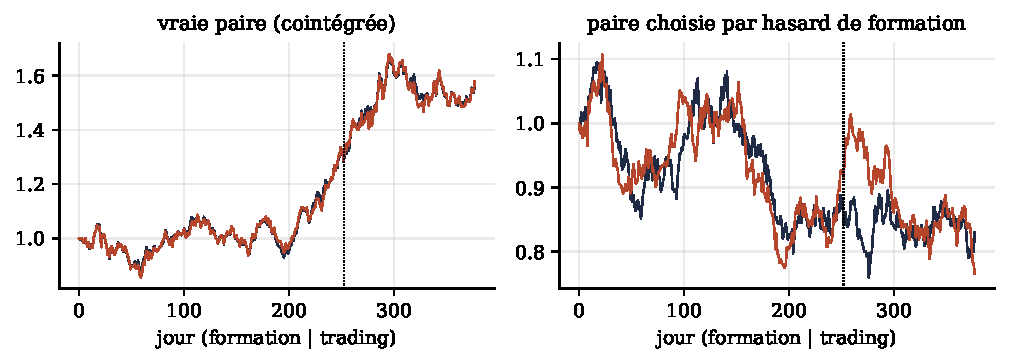
\includegraphics[width=0.95\textwidth]{ch06/ggr_paires.pdf}
\caption{Deux paires du top 20 d'une même formation. À gauche, une vraie paire : les trajectoires restent liées après la formation (ligne pointillée). À droite, une paire retenue parce qu'elle s'est suivie par hasard pendant la formation : elle diverge ensuite.}
\label{c6:fig:pairs}
\end{figure}

\paragraph{Ce que montrent les chiffres.} (1) La SSD classe bien les vraies paires en tête, mais le portefeuille de 20 paires dilue leur profit avec celui de paires fictives qui perdent de l'argent ; c'est pourquoi les 5 ou 10 premières paires font beaucoup mieux que les 20. (2) Les coûts détruisent vite un avantage de quelques dixièmes de pour cent par semestre : à 10 pb par jambe, la stratégie perd de l'argent. (3) Même sans coûts, un tiers des semestres sont perdants.

% =====================================================================
\section{Pourquoi la SSD est un critère imparfait}
% =====================================================================

Développons la SSD. En notant $D_t = \tilde P_{i,t} - \tilde P_{j,t}$ et $\bar D$ sa moyenne sur la formation,
\[
\frac{1}{T_f}\mathrm{SSD}_{ij} = \frac{1}{T_f}\sum_t D_t^2 = \bar D^2 + \widehat{\Var}(D).
\]
Minimiser la SSD revient donc à choisir des paires dont l'écart est petit en moyenne \emph{et peu variable}. Or un \emph{pairs trade} gagne à chaque aller-retour environ deux écarts-types de l'écart (chapitre~1) : une paire à l'écart très peu variable gagne très peu par trade et peine à couvrir ses coûts. La paire idéale a au contraire un écart \emph{ample} et qui revient \emph{vite} à la moyenne : la SSD ne mesure ni l'un ni l'autre \citep{krauss2017survey}.

\begin{pitfall}
La SSD minimale est atteinte par deux actions identiques, par exemple deux lignes de cotation de la même société, ou deux ETF sur le même indice : l'écart est nul, il n'y a rien à gagner. À l'inverse, deux actions qui oscillent fortement l'une autour de l'autre (très bon candidat) ont une SSD plus élevée et peuvent être écartées. Le critère de sélection et le critère de profit ne sont pas les mêmes.
\end{pitfall}

\paragraph{Améliorations proposées.} Restreindre la recherche au même secteur ou sous-secteur \citep{dofaff2012} ; exiger un nombre minimal de croisements de l'écart pendant la formation (indicateur direct de retour à la moyenne) ; combiner distance et test de cointégration \citep{huck2009,rad2016} ; normaliser l'écart par sa volatilité, ce qui conduit au \emph{z-score} du chapitre~1.

% =====================================================================
\section{Études de cas réelles}
% =====================================================================

On applique la règle GGR à nos deux paires réelles : formation sur les 252 premières séances, trading sur les 248 suivantes.

\begin{codebox}[ — E4, règle GGR sur données réelles]
\textbf{KO/PEP :} l'écart normalisé a déjà un écart-type de $9{,}6\,\%$ pendant la formation (les deux titres ont divergé). Une seule position est ouverte pendant la période de trading et ne se referme jamais : perte de $24{,}1\,\%$ avant coûts. \textbf{GLD/GLDM :} écart-type de formation de $0{,}135\,\%$ ; une position, gain brut nul ($-0{,}01\,\%$), $-0{,}21\,\%$ après coûts de 5 pb par jambe.
\end{codebox}

\paragraph{Lecture.} KO/PEP illustre le risque central de la méthode : une paire qui ne revient pas, gardée jusqu'à la fin de la période faute de stop-loss. GLD/GLDM illustre l'autre extrême : un écart si petit qu'aucun trade ne couvre ses coûts. Ces deux cas sont les deux faces du problème décrit à la section précédente.

% =====================================================================
\section{Ce que la théorie apporte, et ses limites}
% =====================================================================

\paragraph{Apports.} Un protocole simple et reproductible, une référence pour comparer toutes les autres méthodes, une définition claire du rendement d'une stratégie autofinancée, et la preuve historique qu'un avantage a existé.

\paragraph{Limites.} Pas de modèle de l'écart, donc pas de demi-vie ni de seuil optimal ; ratio de couverture implicite de 1 dollar contre 1 dollar, sans justification statistique ; sélection biaisée vers les écarts peu volatils ; profits historiques en déclin et très sensibles aux coûts, au coût d'emprunt et au décalage d'exécution.

% =====================================================================
\section{Fiche à recopier au tableau blanc}
% =====================================================================

\begin{whiteboard}
\begin{itemize}[leftmargin=1.2em]
\item \textbf{Formation 12 mois :} $\tilde P_{i,t} = P_{i,t}/P_{i,0}$, $\mathrm{SSD}_{ij} = \sum_t(\tilde P_{i,t}-\tilde P_{j,t})^2$, top 20 paires.
\item \textbf{Calcul matriciel :} $\mathrm{SSD} = \mathrm{diag}(G)\mathbf 1^\top + \mathbf 1\mathrm{diag}(G)^\top - 2G$, $G = \tilde P^\top\tilde P$.
\item \textbf{Trading 6 mois :} ouvrir à $|D_t| > 2\hat\sigma$ (1\,\$ long / 1\,\$ court), fermer au croisement.
\item \textbf{Gain d'un trade :} $(P^L_{t_1}/P^L_{t_0}-1) - (P^C_{t_1}/P^C_{t_0}-1)$.
\item \textbf{Capital engagé :} somme des gains / 20 ; \textbf{employé :} / nombre de paires ouvertes.
\item \textbf{Biais de la SSD :} $\mathrm{SSD}/T = \bar D^2 + \widehat\Var(D)$ : favorise les écarts peu volatils.
\end{itemize}
\end{whiteboard}

% =====================================================================
\section{Exercices}
% =====================================================================

\begin{exercise}
Démontrez l'identité $\frac1T\sum_tD_t^2 = \bar D^2 + \widehat\Var(D)$ (avec la variance empirique divisée par $T$).
\end{exercise}

\begin{exercise}
Une paire a un écart de formation d'écart-type $1\,\%$. Les coûts sont de 5 pb par jambe et par transaction. Quel gain minimal (en écarts-types) doit capturer un aller-retour pour être rentable ?
\end{exercise}

\begin{exercise}[à coder]
Ajoutez à \texttt{trade\_pair} un décalage d'exécution d'un jour (signal en $t$, exécution en $t+1$) et un stop-loss à $4\hat\sigma$. Mesurez l'effet de chacun sur les vraies et les fausses paires.
\end{exercise}

\begin{exercise}[à coder]
Remplacez le critère SSD par : SSD minimale \emph{parmi les paires du même secteur ayant au moins 8 croisements pendant la formation}. La part de vraies paires dans le top 20 augmente-t-elle ? Et le rendement ?
\end{exercise}

% =====================================================================
\section{Pour aller plus loin}
% =====================================================================

\begin{toread}
\begin{itemize}[leftmargin=1.2em]
\item \citet{gatev2006} : la section sur la méthodologie (formation, trading, calcul des rendements) et les tests de robustesse au décalage d'exécution.
\item \citet{dofaff2010,dofaff2012} : l'évolution des profits dans le temps et l'effet des coûts.
\item \citet{krauss2017survey}, la partie consacrée à l'approche par distance : synthèse des variantes et de leurs critiques.
\end{itemize}
\end{toread}

\section{Scripts du chapitre}
\noindent\texttt{code/ch06/ch06\_distance\_method.py} : E1–E3 (protocole GGR simulé, figure~\ref{c6:fig:pairs}), E4 (données réelles). Univers : \texttt{code/common/universe.py}.
